\section{The Blobs module}

\ToDo{[Miguel]: the English at this section is bad, and some parts are vage or difficult to follow. It needs a rewrite.}

\subsection{Introduction}
\label{sec:blobs_introduction}
\ToDo{[Miguel]: this should be moved to a more general section, about the current system.}
Necessarily, management of this part is very important. Nowadays, each demo owns images.
Even if they are not heavy (minus 1 MB),
when there are fifty different demos on system and each demo is downloaded using
\emph{GitHub} \cite{GitHub} then the compilation of system takes too much time.
Knowing that each
demo details a mathematic theory with complex calculations and several demos use
same images, it will be preferable to create a system to manage theses images. \\
\setlength{\parindent}{0cm}

Before specifing this abstract system, it must be known with precision how the actual system
works.\\
\setlength{\parindent}{0cm}

According to the provided UML (\ref{img:IPOL_diagram_class}), one class "image" implements
functions changing image characteristics. To do it, it uses \emph{PIL} \cite{PIL}.
Images have two formats: thumbnail and an input image. Thumbnail allows the user visualize
and select an input image on client side. Input image is which use to apply algorithm on it,
algorithm specific to the demo. This part is made in the implementation of demo.
Moreover, configuration file allows to customize the default input files.
The images are stored in a directory ("/input"). When using client side of the demo to test
it, new images are generated and stored in a temporary directory in ("/tmp").\\
\setlength{\parindent}{0cm}

\begin{figure}[H]
  \centering
  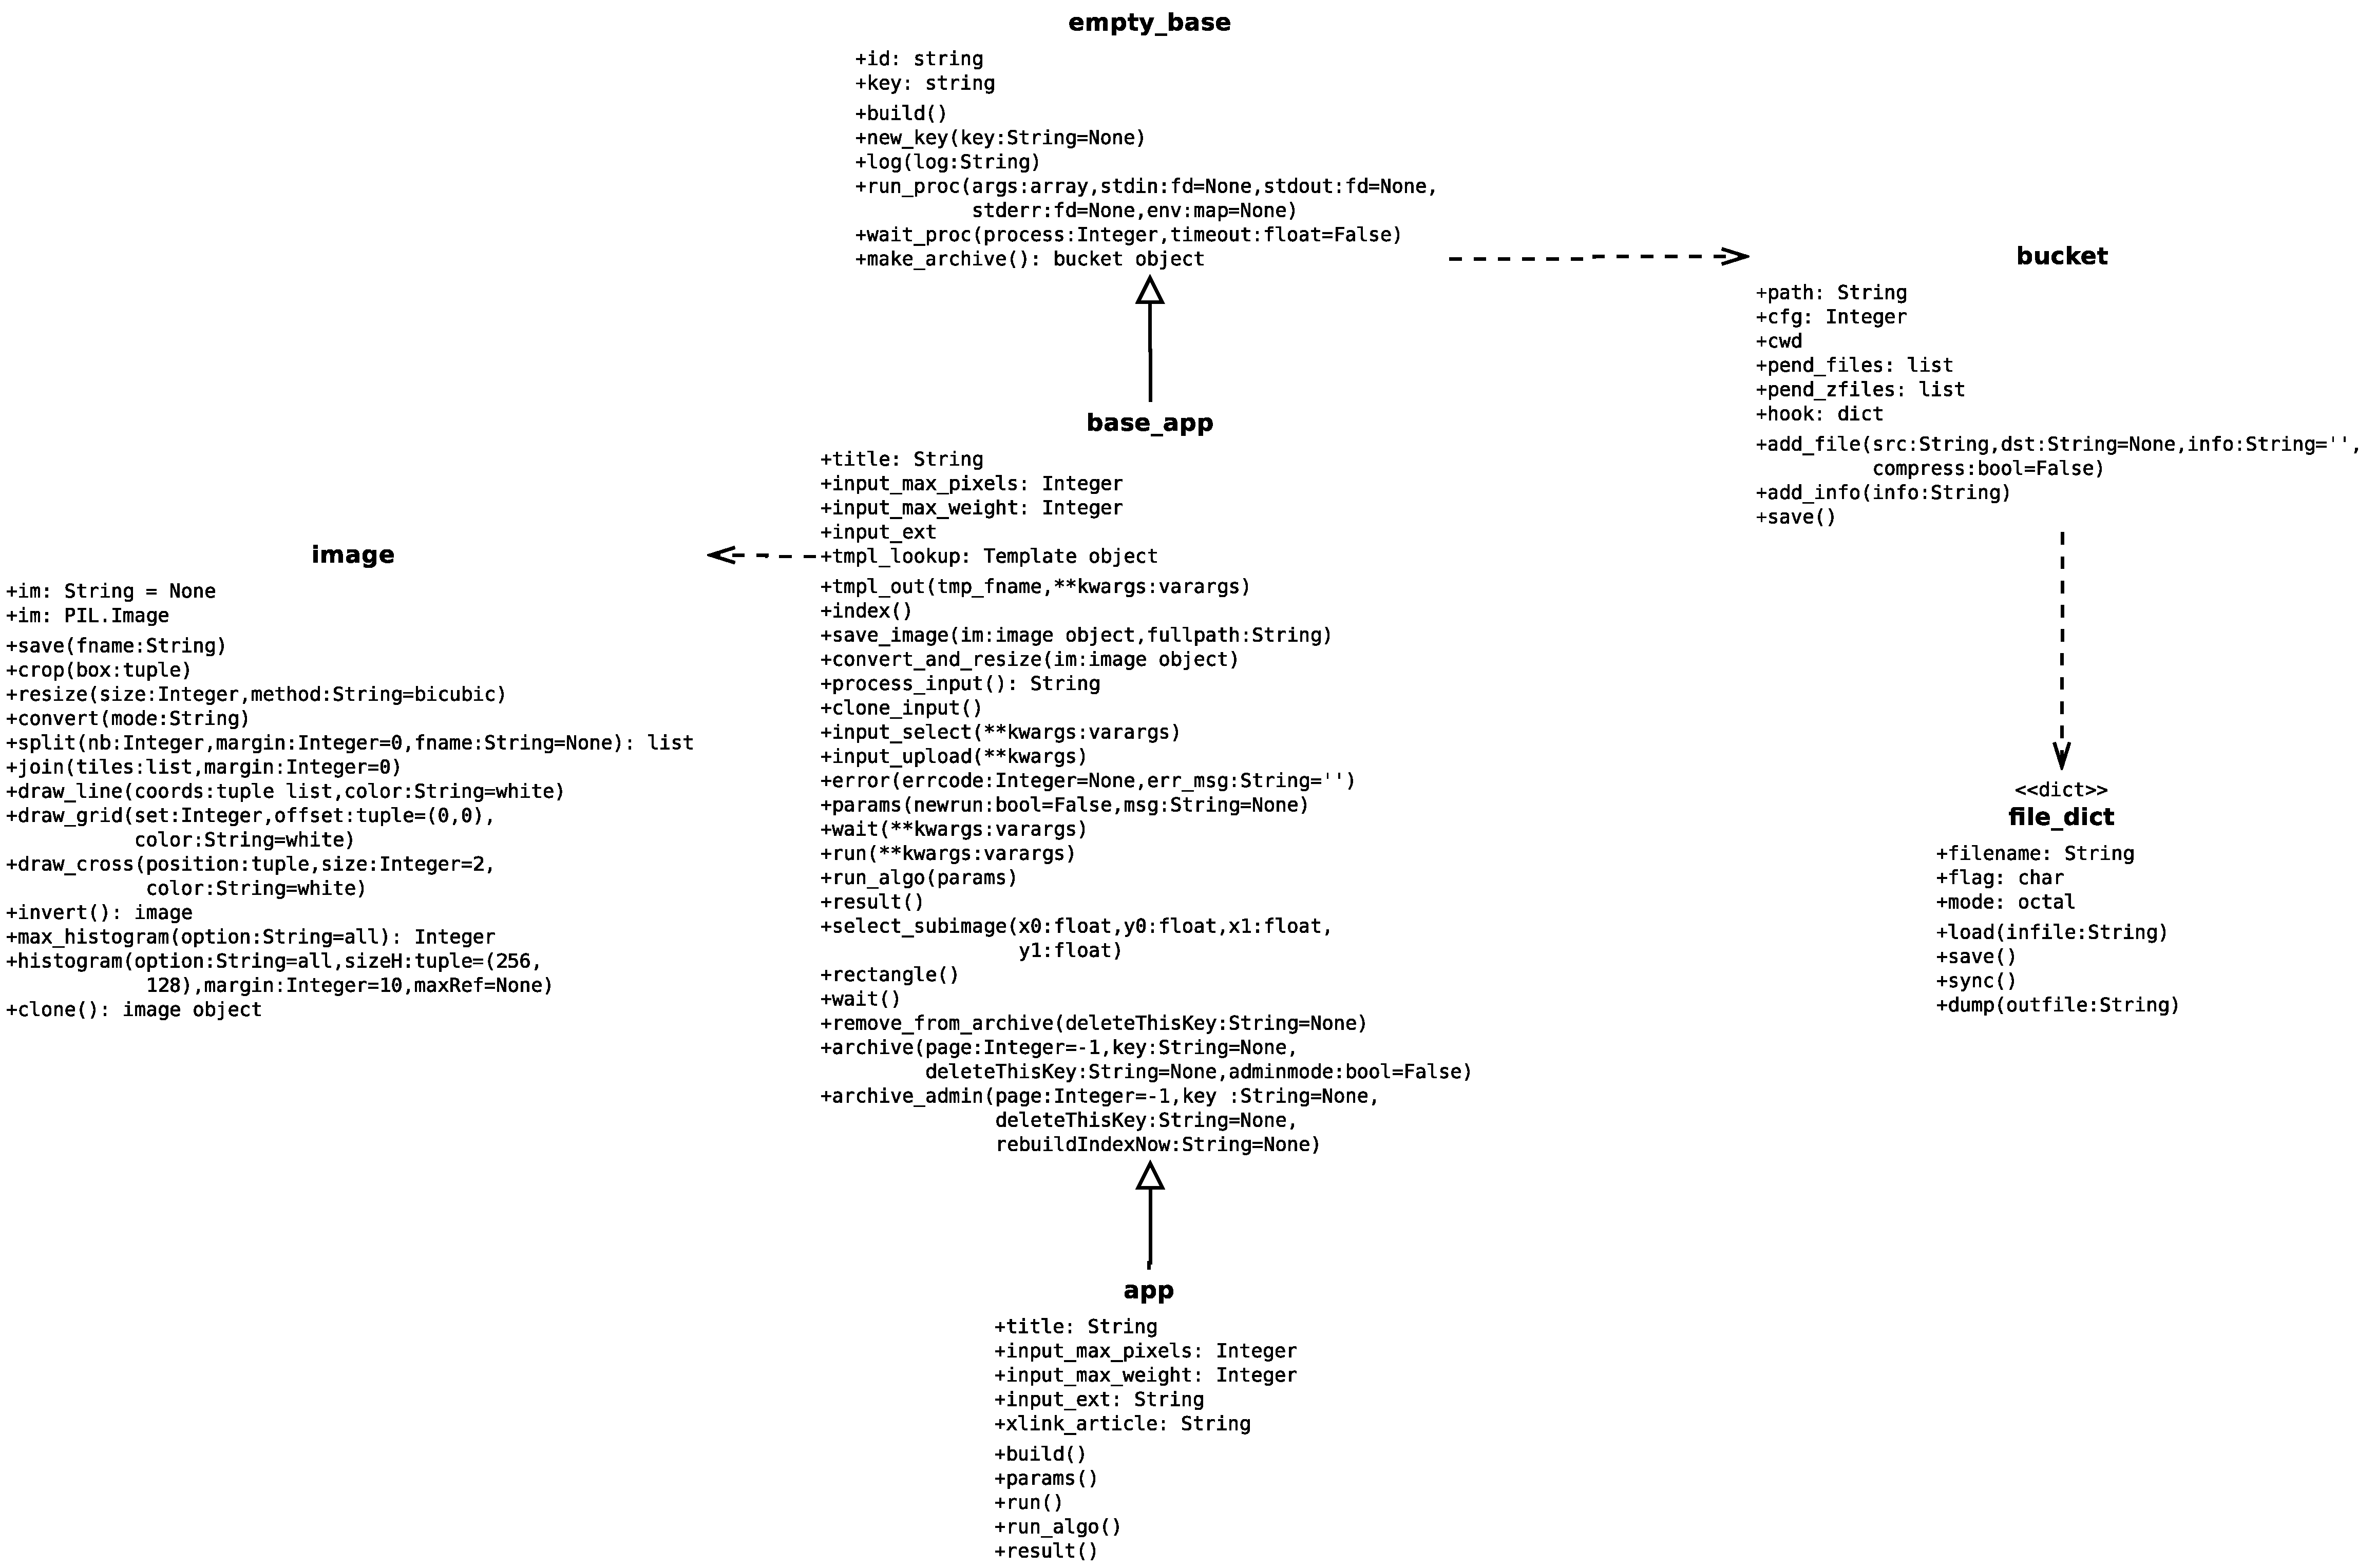
\includegraphics[width=20.0cm, angle=90]{blobs/images/IPOL_diagram_class.pdf}
  \caption{UML diagram class of current system. \ToDo{[Miguel]: this should be moved to a more general section.}}
  \label{img:IPOL_diagram_class}
\end{figure}

To conclude this part, images are result of demo and the management of these is important
for the project.

\subsection{Demo}
\ToDo{[Miguel]: this should be moved to a more general section, about the current system.}
During introduction, demo system will claim like "God Object". It is excessive term in
order to represent the system with a metaphor. It is just a complex object.
In this section, it will detail functionalities to clarify objective thereof and
look how it is possible to improve it.\\
\setlength{\parindent}{0cm}

Firstly, this object introduce here (\ref{img:IPOL_diagram_class}), has many ways to
interact with user. It implements all features of project. For example, it manages
interaction with client side. To do so, it is a part of webserver developed in
\emph{CherryPy} \cite{CherryPy}.
Communication between the client and the server is done using an
\emph{HTTP} \cite{HTTP}. Indeed, when users call a functionality,
this object allows to search the expected result. For example, when users call an algorithm,
it runs the corresponding binary in "bin/" file, manage images archiving the result
and call the HTTP response using the \emph{Mako Template Library} \cite{Mako}.
Knowing these possibilities, it is very difficult to add new functionalities to this object.
\\
\setlength{\parindent}{0cm}

To conclude this part, the demo is a powerful object but to go further, it needs to create
separate module which communicate with the core system.

\subsection{Solution}
\setlength{\parindent}{1cm}
\hspace{1cm}

Since the problematic have been detailled, it will be necessary to solve it. In this part,
it will present to you \textbf{MVC pattern}, \textbf{Factory pattern}, \textbf{Database}.
\ToDo{[Miguel]: the Factory pattern is not used, but it can be discussed why.}

\subsubsection{MVC pattern}
\setlength{\parindent}{1cm}
\hspace{1cm}

\ToDo{[Miguel]: this should be moved to a more general section.}

MVC, alias Model-View-Controller, is architectural pattern used in interface implementation.
It consists of create three separates parts. The model manage database and it is observable
object. The aim of view is to update data from model and to notify event, which by user,
to controler. The controler receive notification from view and update the model.
\setlength{\parindent}{0cm}
In our case, the model will be protocol used to interact with database of images.
The view is client side which look by users using them browser.
It will be updates in the control of the web page on client side.
The controler will be the code used to manage new module implementing functionalities.



\begin{figure}[H]
  \centering
  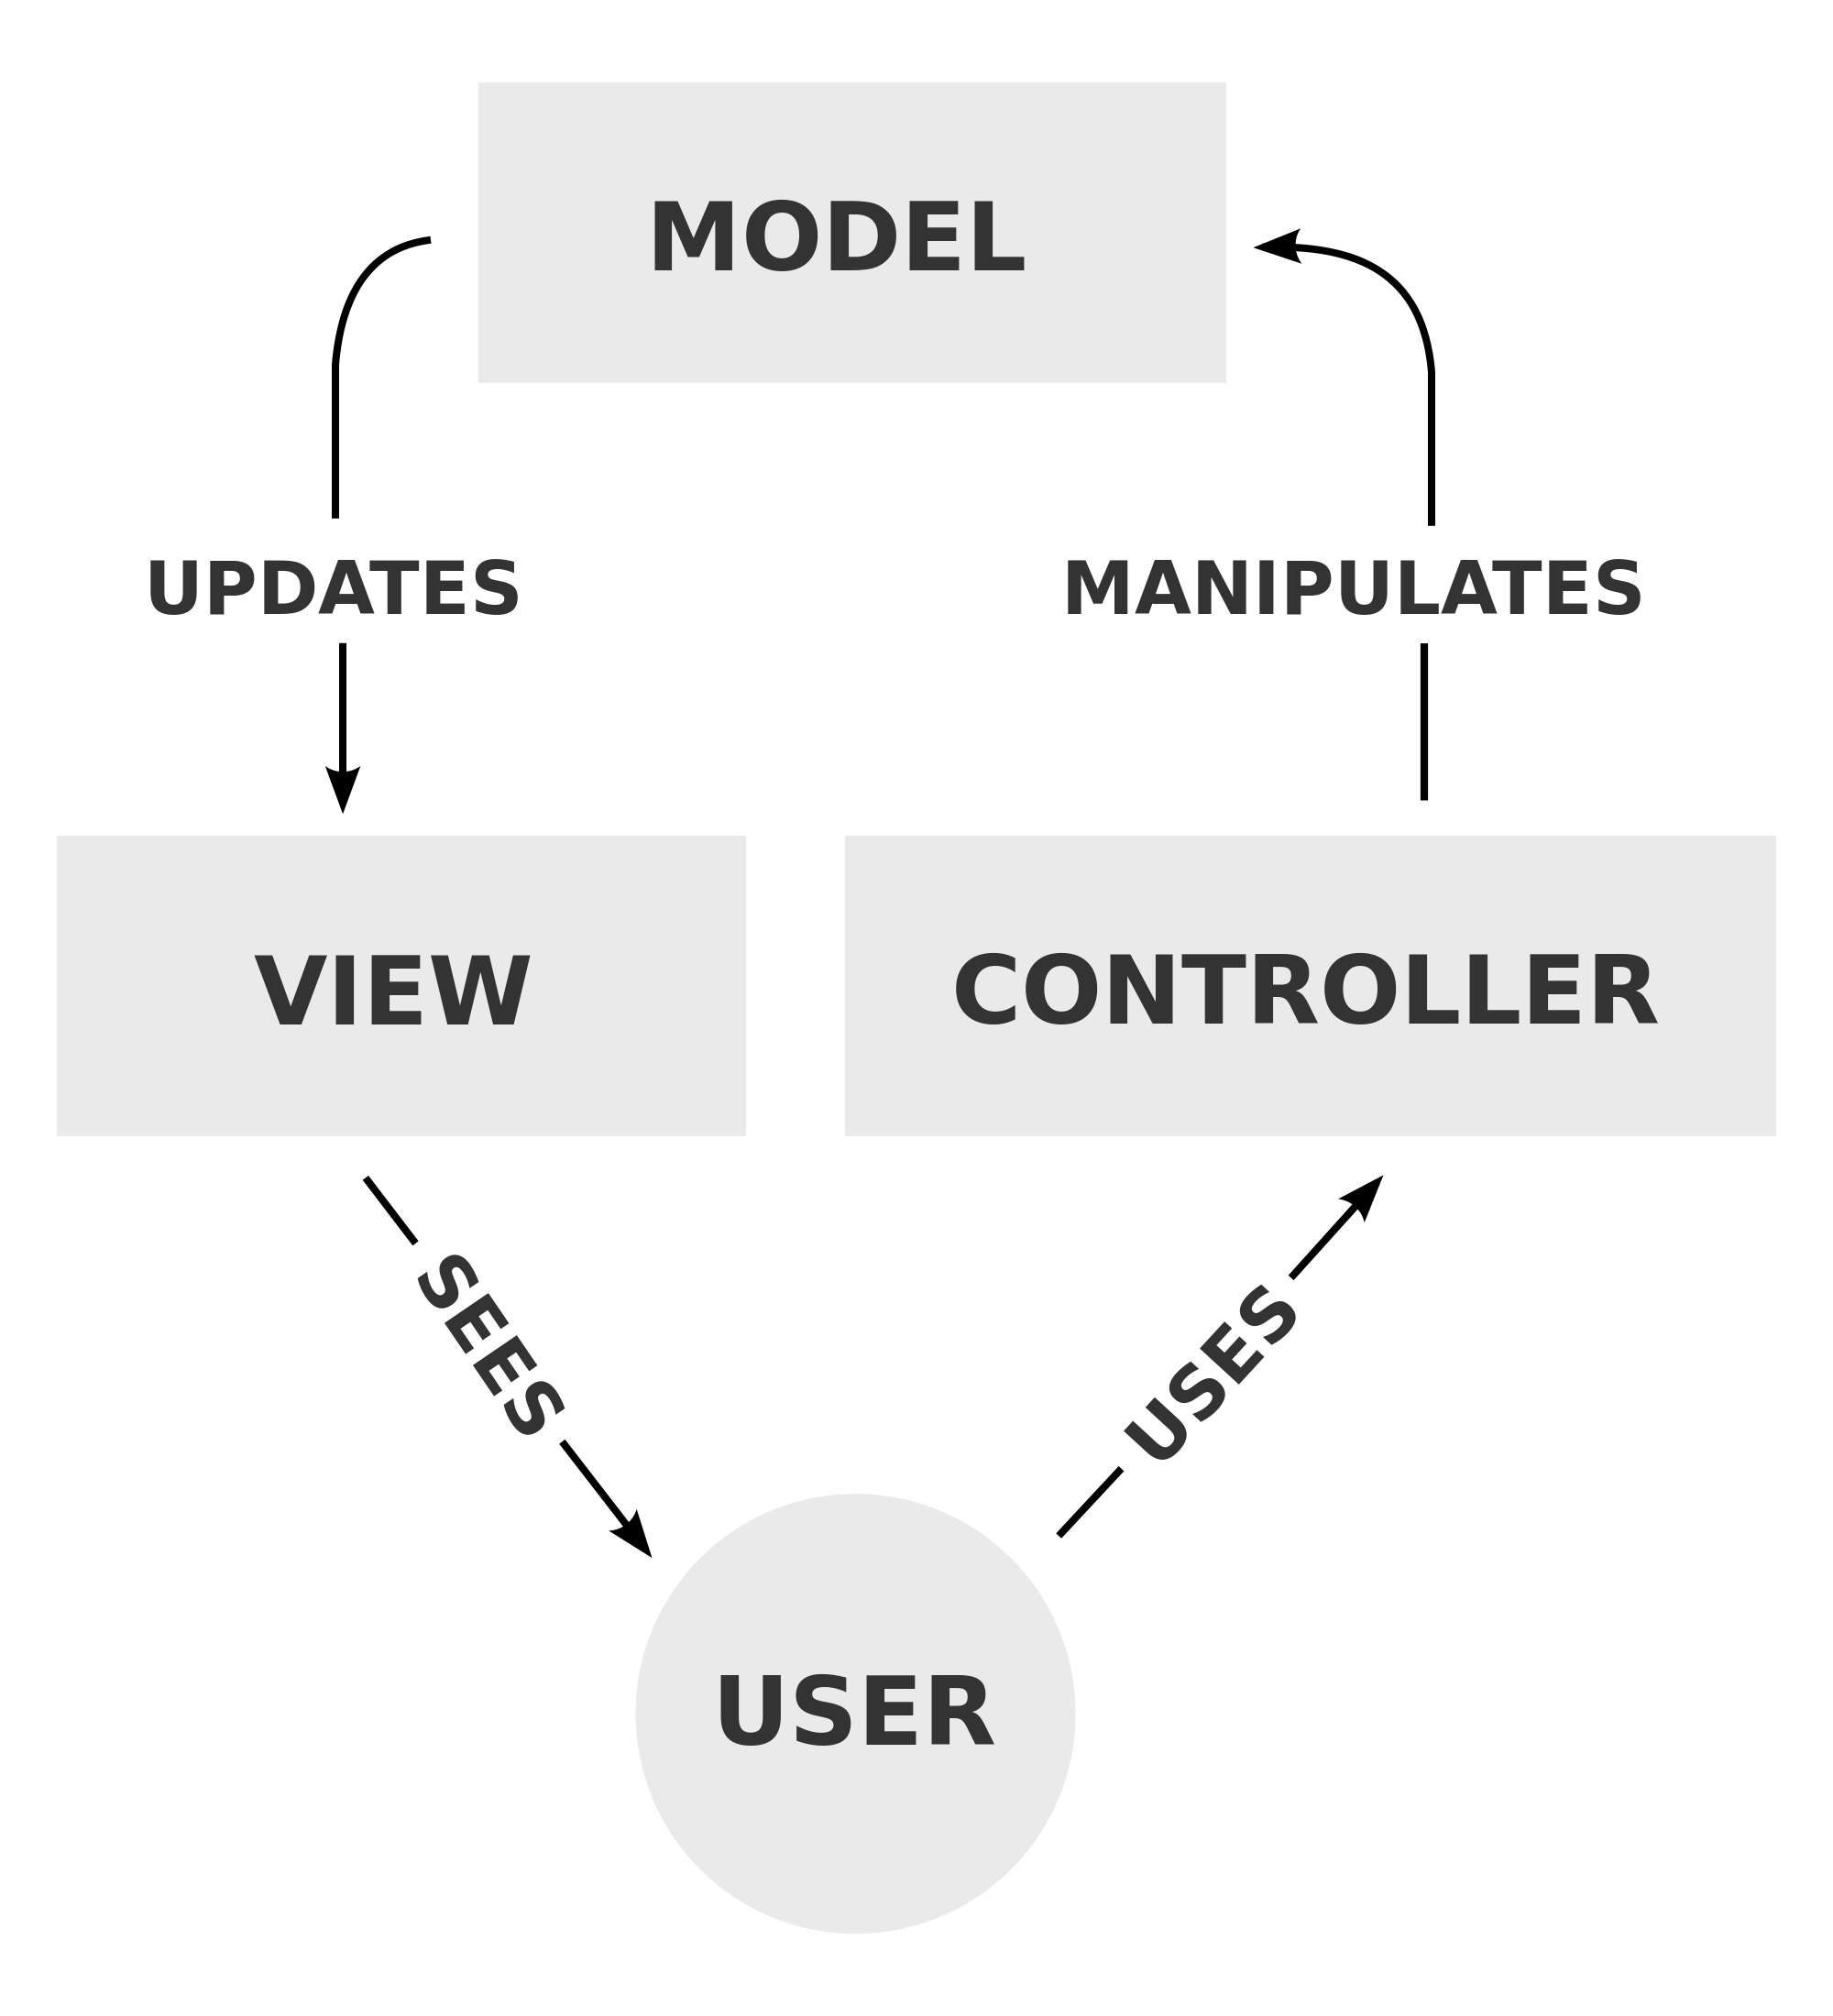
\includegraphics[width=3.5in]{blobs/images/MVC-Process}
  \caption{The MVC pattern}
  \label{img:MVC-Process}
\end{figure}

\begin{comment}
\subsubsection{Factory pattern}
\setlength{\parindent}{1cm}
\hspace{1cm}
\ToDo{[Miguel] The factory pattern is not used in the new system, since finally
backwards compatibility needs not to be ensure. 
This section should be removed.}

Factory is a \textbf{design pattern\footnote{\cite{GoF}}} allowing to create other objects.
In order to explain the Factory pattern, it must know what is an inheritance.
In inheritance based on object-oriented
programming, it is possible to create an interface (or abstract class) which two different
classes inherit. The most famous example should be the interface Animal which is defined that
Animal could have and it must have to be animal. Dog and Cat are two different classes
inheriting each one from Animal class.
Factory, in this case, could be Farm class. In function to the type of animal which you want
to create (ex: 1 for Cat and 2 for Dog), the Farm will instantiated one of two ways like
Animal class. To do that, it can use implicit or specific cast, it depends of language of
programming.
\bigbreak
\setlength{\parindent}{0cm}
In our case, it will have two versions of demos. The first one like it is nowadays, and the
second one which will be interact with new module. The aim factory is to create just one
object instantiating one of two ways. Consequently, it will be easier to make it work both
version on the same system.

\begin{figure}[H]
  \centering
  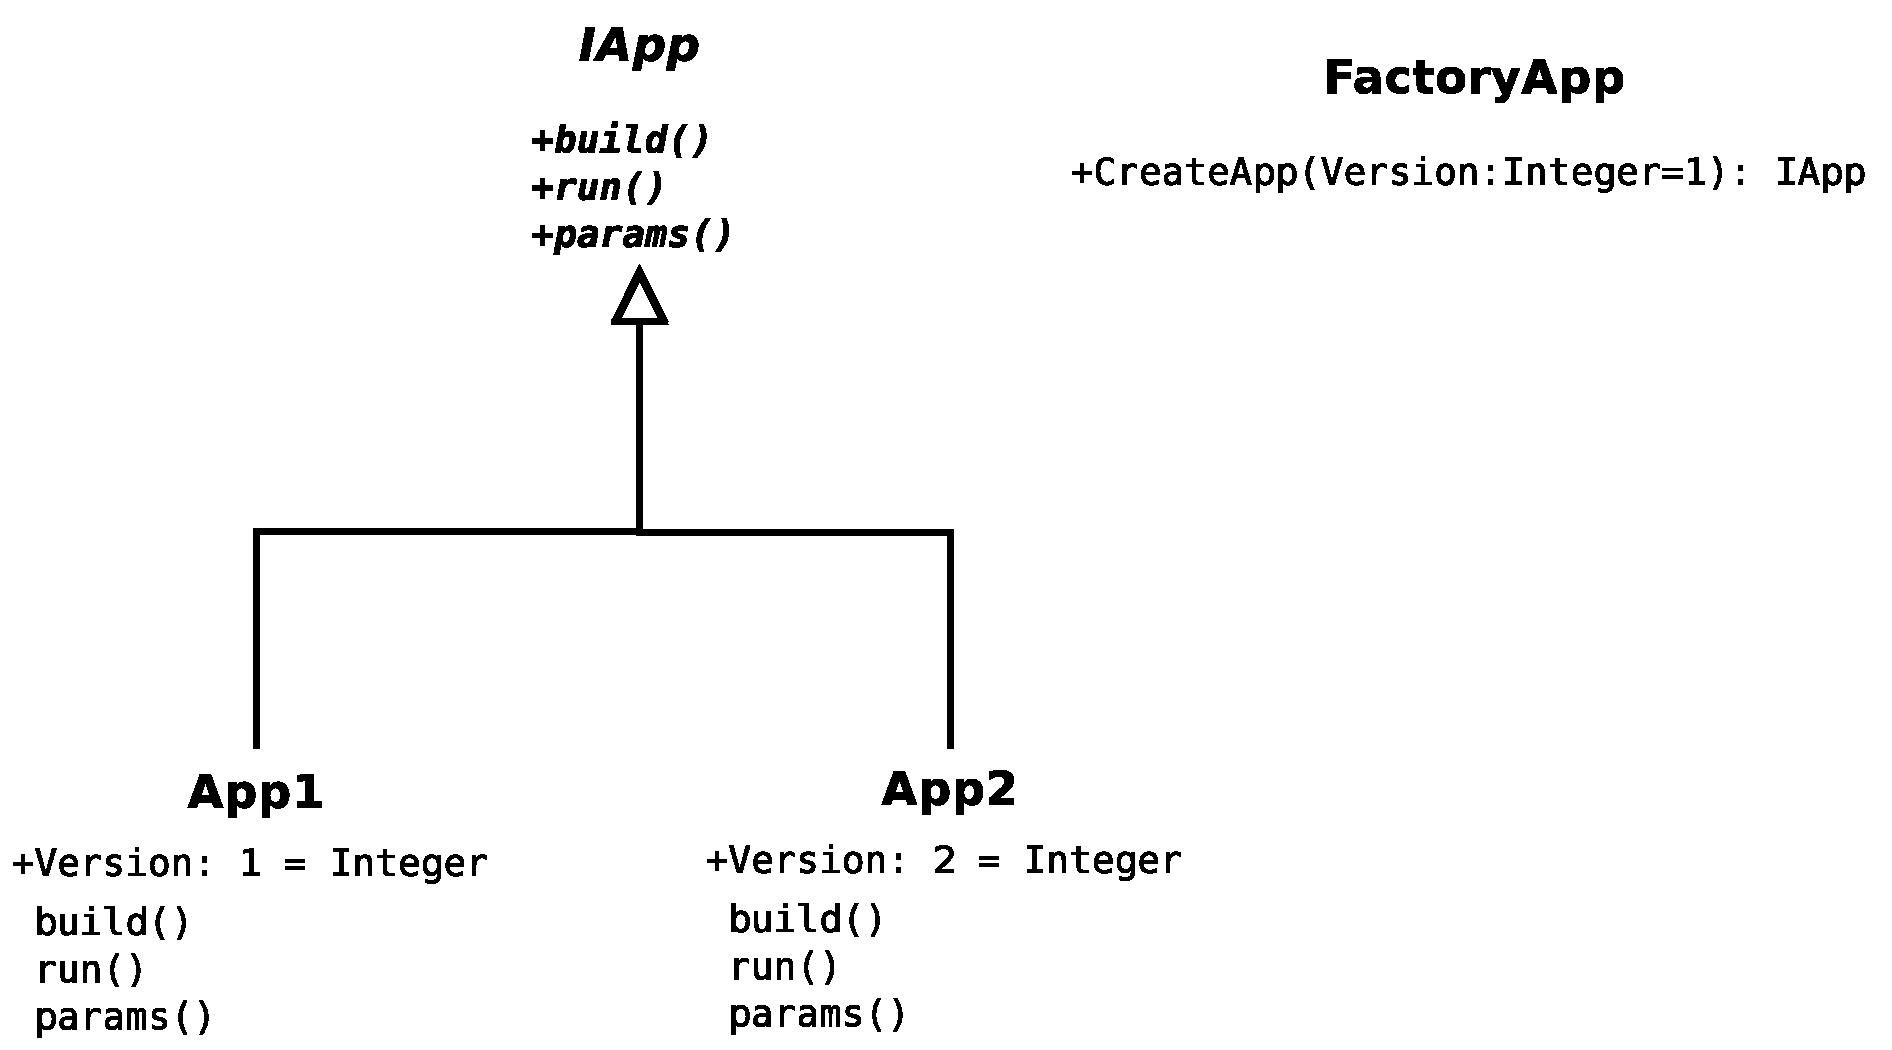
\includegraphics[width=5in]{blobs/images/Example_Factory_Pattern}
  \caption{An example of Factory pattern}
  \label{img:Example_Factory_Pattern}
\end{figure}
\end{comment}

\subsubsection{Database}
\ToDo{[Miguel] Check that the database information in this section is correct and up to date}

\ToDo{[Miguel] It seems that we should have a foreign key in the table \emph{demo} for field \emph{template\_id}. Without it, it could be possible to have a demo which uses the blobs of a non-existing demo.}

We use a SQL database to help managing blobs, that can contain images or other 
type of data needed as inputs for the demos.
It will use a back-end and will be created with \emph{SQLite} \cite{SQLite}.
Figure \ref{img:images_bdd} depicts the different tables, their contents and their
relations.

\begin{figure}[H]
  \centering
  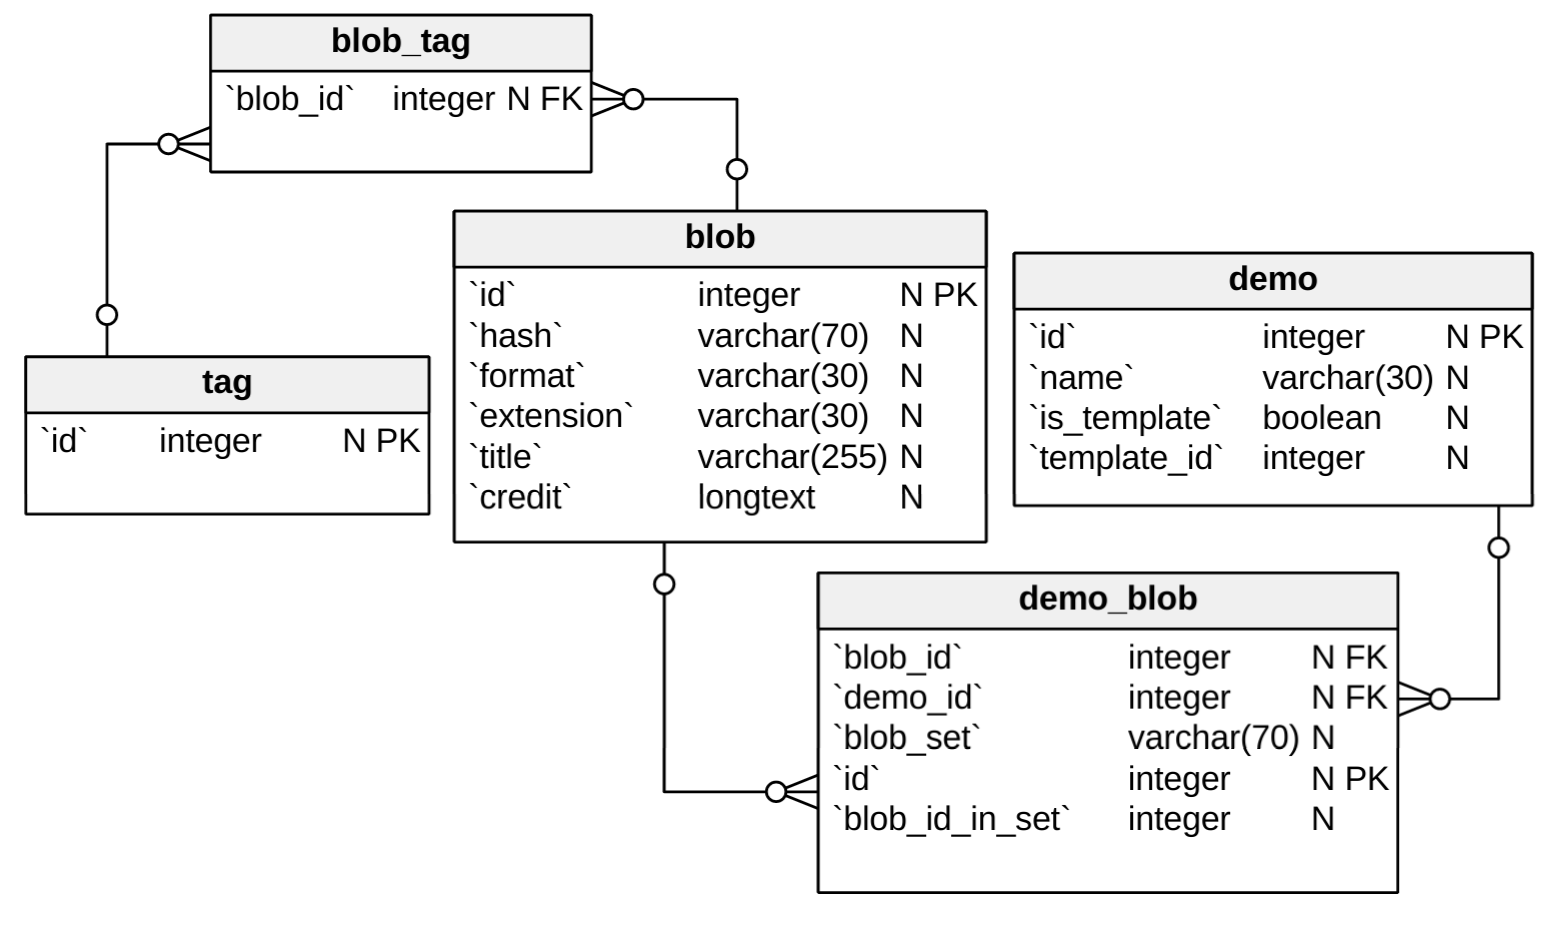
\includegraphics[width=\textwidth]{blobs/images/images_bdd_vertabelo}
  \caption{Database schema for the Blobs module. \ToDo{[Miguel] This diagram was made with Verbatelo. Is there any free software and automatic tool to use instead? It needs to be a vectorial graphic, not raster. In general, using an automatic tool which creates automatically the diagram is a very good idea. Also: missing \emph{name} inside table \emph{tag}. An automatic tool will avoid that we forget to add fields, since the diagram will be generated automatically.}}
  %\footnotesize
  %\caption*{Realized with MySQL Workbench}
  \label{img:images_bdd}
\end{figure}


\subsection{Remarks}
\subsubsection{Concurrent accesses}
\setlength{\parindent}{1cm}
\hspace{1cm}
\ToDo{[Miguel]: this should be moved to a more general section, because it applies to all modules.}
The library used to insert, select or update database is
\emph{SQLite} \cite{SQLite}. This thereof manages, internally,
the concurrent access to database. Indeed, when two people want to
access to the database: the first one will do his request while
the other will be locked by mutex. This principle is also used by transactions
(BEGIN or END/COMMIT).
Therefore, at the beginning of development, it was thought only need a
connection to the database.\\
The problem of the concurrent accesses has been raised during errors occured.
Indeed, when errors occured, the program throws exception and call "roll back"
database's function. Imagine that some people try access to the same data and to
modify it, but some successed it and some failed. The problem of using a only
connection is how to know what changes have been taken into account knowing
that for certain, the database rolled back.\\
Therefore for each request requiring the database,
a new instance (new connection) is used. Thus, the problems
of "roll back" are avoided. Nevertheless, it would be preferable to use a decorator
to avoid the redundance of the code.

\subsubsection{Consistency check}
\ToDo{[Miguel]: this should be moved to a more general section.}

The consistency check in database management system (DBMS) is the fact
to verify the consistency between the information present on hard disk and
those present on database.\\
There are two ways to do this: running database consistency check manually and
automatically. The program uses consistency check manually in order to
having the control on the error occuring.\\
That is why, when the program uses the action database (SELECT, DELETE, UPDATE),
each information is checked. If errors occurs, an database's exception is caught
and custom exception is throwed to called function.
The consistency check manually is also used because the design databse
has some constraints like: "DELETE CASCADE" and "UPDATE RESTRICT".

\subsubsection{Reference of the module services}
\ToDo{Some of the information here is inconsistent with the actual API implemented in the module. Fix it.}
\ToDo{Think of a better way to describe the webservice API, rather than a table. We need to have homogeneity in the documentation. The format of the Archive module seems better.}

\begin{flushleft}
\begin{longtable}
                   {|C{\dimexpr 0.2\linewidth-2\tabcolsep}
                    L{\dimexpr 0.8\linewidth-2\tabcolsep}|}
% {|C{\dimexpr 0.30\linewidth-2\tabcolsep}||
%                     C{\dimexpr 0.20\linewidth-2\tabcolsep}|
%                     C{\dimexpr 0.18\linewidth-2\tabcolsep}|
%                     C{\dimexpr 0.32\linewidth-2\tabcolsep}|}
%   \hline
%   {\bf Function Name} & {\bf Description} & {\bf Param.} & {\bf Return} \tabularnewline
  \hline
  \multicolumn{2}{|l|}{\textbf{add\_blob\_ws}(demo\_id, path, tag, ext, the\_set, title, credit)} \\ 
                  & add blob to database \\
                  & {\{  return:OK or KO, the\_hash: ...  \}} \\
  \hline
  \multicolumn{2}{|l|}{\textbf{add\_demo\_ws}(name, is\_template, template)} \\ 
                  & add demo to database \\
                  & { \{ return:OK or KO \} }\\
  \hline
  \multicolumn{2}{|l|}{\textbf{add\_tag\_to\_blob\_ws}(blob\_id, tag)} \\ 
                  & add tag to database \\
                  & { \{ return:OK or KO \} }\\
  \hline
  \multicolumn{2}{|l|}{\textbf{delete\_blob\_ws}(demo\_id, blob\_id)} \\ 
                  & delete blob from id demo and id blob \\
                  & { \{ return:OK or KO, delete: (hash, extension) \}} \\
  \hline
  \multicolumn{2}{|l|}{\textbf{demos\_ws}()} \\ 
                  & list demos present  in database \\
                  & {\{ status:OK or KO,
                        list\_demos:  \{ id:int, mame:str, is\_template:int, template\_id:int \} \}} \\
  \hline
  \multicolumn{2}{|l|}{\textbf{get\_blob\_ws}(blob\_id)} \\ 
                  & return blob information from id \\
                  &  {\{ return:OK or KO,
                        \{id, hash,  extension, credit \} \} }\\
  \hline
  \multicolumn{2}{|l|}{\textbf{get\_blob\_url\_ws}(blob\_hash, blob\_ext)} \\ 
                  & return the url link of the blob based on its hash and extension \\
                  &  \{ blob\_url: string that contains the url link of the blob \} \\
  \hline
  \multicolumn{2}{|l|}{\textbf{get\_blobs\_from\_template\_ws}(template)} \\ 
                  & list blobs from name template \\
                  & { \{ return:OK or KO,
                        blobs: \{id, hash,  extension, format \} \} }\\
  \hline
  \multicolumn{2}{|l|}{\textbf{get\_blobs\_of\_demo\_by\_name\_ws}(demo\_name)} \\ 
                  & list blobs from demo name \\
                  & { \{ return:OK or KO,
                        blobs: \{id, hash,  extension, format \},
                        use\_template: \{id: name, is\_template, id\_template\}\},
                        url: 'blob path url',
                        url\_thumb: 'blob thumb path url',
                        physical\_location : 'blob path physical location'
                    }\\
  \hline
  \multicolumn{2}{|l|}{\textbf{get\_blobs\_of\_demo\_ws}(demo)} \\ 
                  & list blobs from demo id \\
                  & { \{ return:OK or KO,
                        blobs: \{id, hash,  extension, format \},
                        use\_template: \{id: name, is\_template, id\_template\}\}}\\
  \hline
  \multicolumn{2}{|l|}{\textbf{get\_tags\_ws}(blob\_id)} \\ 
                  & return list tags from blob id \\
                  & { \{ \{id: name\} \} }\\
  \hline
  \multicolumn{2}{|l|}{\textbf{get\_template\_demo\_ws}()} \\ 
                  & return list demos templated \\
                  &  {\{ return:OK or KO, list\_template: \{id: name\} \}} \\
  \hline
  \multicolumn{2}{|l|}{\textbf{op\_remove\_demo\_ws}(demo\_id)} \\ 
                  & remove demo from id demo  \\
                  & { \{ return:OK or KO \} }\\
  \hline
  \multicolumn{2}{|l|}{\textbf{remove\_tag\_from\_blob\_ws}(id, tag\_id, blob\_id)} \\ 
                  & remove tag for a blob from id tag and id blob  \\
                  & { \{ return:OK or KO \} }\\
  \hline
  \multicolumn{2}{|l|}{\textbf{set\_template\_ws}(demo\_id, id, name)} \\ 
                  & change the current template used by a demo \\
                  & { \{ return:OK or KO \} }\\
  \hline
\end{longtable}
\end{flushleft}


